\newcommand{\adwareTagResultsAucTable}{
    \begin{table}[H]
        \centering
        \begin{tabular}{|p{2,8cm}||p{2,8cm} p{2,8cm} p{2,8cm}|}
            \hline
            Adware Tag & ALOHA & Joint Embedding & Proposed Model \\
            \hline
            AUC-ROC & 0.665$\pm$0.018 & \textBF{0.677$\pm$0.028} & 0.637$\pm$0.024 \\
            \hline
        \end{tabular}
        \caption{AUC-ROC (Area Under Curve) of the different models for the \textbf{Adware Tag} prediction task. Results were aggregated over \textBF{3} training runs with different weight initializations and minibatch orderings. Best results are shown in \textbf{bold}.} \label{tab:adwareTag_auc}
    \end{table}
}

\newcommand{\adwareTagResultsAtFprTable}{
    \begin{center}
        \begin{longtable}[c]{|p{3,2cm}||p{1,8cm} p{1,8cm} p{1,8cm} p{1,8cm} p{1,8cm}|}
            \hline
            Adware Tag & \multicolumn{5}{c|}{{FPR}} \\
            & $10^{-5}$ & $10^{-4}$ & $10^{-3}$ & $10^{-2}$ & $10^{-1}$ \\
            \hline
            \endfirsthead

            \caption*{\raggedright ...continued from previous page} \\
            \hline
            Adware Tag & \multicolumn{5}{c|}{\textbf{FPR}} \\
            & $10^{-5}$ & $10^{-4}$ & $10^{-3}$ & $10^{-2}$ & $10^{-1}$ \\
            \hline
            \endhead

            \caption*{\raggedleft ...continued on next page} \\
            \endfoot

            \caption{Mean and standard deviation results (TPR, Accuracy, Recall, Precision and F1-Score) of the different models for the \textbf{Adware Tag} prediction task at different \textbf{FPR}s (\textit{False Positive Rates}). Results were aggregated over \textBF{3} training runs with different weight initializations and minibatch orderings. Best results are shown in \textbf{bold}. Under \textbf{TPR} results are also presented the percentage reduction in mean detection error and in ROC curve standard deviation introduced by the \textit{Proposed Model} with respect to both \textit{ALOHA} model and \textit{Joint Embedding}.} \label{tab:adwareTag_results_at_fpr} \\
            \endlastfoot

            \multicolumn{6}{|c|}{\textbf{TPR}} \\
            \hline
            ALOHA & \textBF{0.003$\pm$0.004} & \textBF{0.003$\pm$0.004} & 0.003$\pm$0.004 & 0.009$\pm$0.000 & \textBF{0.139$\pm$0.066} \\
            Joint Embedding & 0.002$\pm$0.002 & 0.002$\pm$0.002 & \textBF{0.003$\pm$0.002} & \textBF{0.033$\pm$0.012} & 0.088$\pm$0.004 \\
            Proposed Model & 0.002$\pm$0.002 & 0.002$\pm$0.002 & \textBF{0.003$\pm$0.002} & 0.024$\pm$0.012 & 0.095$\pm$0.013 \\
            \hline
            Error Reduction wrt \newline ALOHA & -0.1\% & -0.1\% & 0.0\% & 1.5\% & -5.1\% \\
            Error Reduction wrt \newline Joint Embedding & 0.0\% & 0.0\% & 0.0\% & -0.9\% & 0.8\% \\
            \hline
            Std Reduction wrt \newline ALOHA & 50.0\% & 50.0\% & 50.0\% & 0.0\% & 80.3\% \\
            Std Reduction wrt \newline Joint Embedding & 0.0\% & 0.0\% & 0.0\% & 0.0\% & -225.0\% \\
            \hline
            \multicolumn{6}{|c|}{\textbf{Accuracy}} \\
            \hline
            ALOHA & \textBF{0.910$\pm$0.000} & \textBF{0.910$\pm$0.000} & 0.909$\pm$0.002 & 0.902$\pm$0.000 & \textBF{0.831$\pm$0.007} \\
            Joint Embedding & \textBF{0.910$\pm$0.000} & \textBF{0.910$\pm$0.000} & \textBF{0.910$\pm$0.000} & \textBF{0.905$\pm$0.001} & 0.827$\pm$0.005 \\
            Proposed Model & \textBF{0.910$\pm$0.000} & \textBF{0.910$\pm$0.000} & \textBF{0.910$\pm$0.000} & 0.904$\pm$0.001 & 0.826$\pm$0.004 \\
            \hline
            \multicolumn{6}{|c|}{\textbf{Recall}} \\
            \hline
            ALOHA & \textBF{0.003$\pm$0.004} & \textBF{0.003$\pm$0.004} & 0.003$\pm$0.004 & 0.009$\pm$0.000 & \textBF{0.139$\pm$0.066} \\
            Joint Embedding & 0.002$\pm$0.002 & 0.002$\pm$0.002 & \textBF{0.003$\pm$0.002} & \textBF{0.033$\pm$0.012} & 0.088$\pm$0.004 \\
            Proposed Model & 0.002$\pm$0.002 & 0.002$\pm$0.002 & \textBF{0.003$\pm$0.002} & 0.024$\pm$0.012 & 0.095$\pm$0.013 \\
            \hline
            \multicolumn{6}{|c|}{\textbf{Precision}} \\
            \hline
            ALOHA & \textBF{1.000$\pm$0.000} & \textBF{1.000$\pm$0.000} & 0.333$\pm$0.471 & 0.086$\pm$0.002 & \textBF{0.118$\pm$0.049} \\
            Joint Embedding & \textBF{1.000$\pm$0.000} & \textBF{1.000$\pm$0.000} & 0.333$\pm$0.236 & \textBF{0.262$\pm$0.066} & 0.080$\pm$0.005 \\
            Proposed Model & \textBF{1.000$\pm$0.000} & \textBF{1.000$\pm$0.000} & \textBF{0.500$\pm$0.408} & 0.196$\pm$0.081 & 0.085$\pm$0.012 \\
            \hline
            \multicolumn{6}{|c|}{\textbf{F1 Score}} \\
            \hline
            ALOHA & \textBF{0.006$\pm$0.008} & \textBF{0.006$\pm$0.008} & 0.006$\pm$0.008 & 0.016$\pm$0.000 & \textBF{0.128$\pm$0.056} \\
            Joint Embedding & 0.003$\pm$0.004 & 0.003$\pm$0.004 & \textBF{0.006$\pm$0.004} & \textBF{0.059$\pm$0.020} & 0.084$\pm$0.004 \\
            Proposed Model & 0.003$\pm$0.004 & 0.003$\pm$0.004 & \textBF{0.006$\pm$0.004} & 0.043$\pm$0.021 & 0.090$\pm$0.013 \\
            \hline
        \end{longtable}
    \end{center}
}

\newcommand{\adwareTagResultsSummaryTable}{
    \begin{table}[H]
        \centering
        \begin{tabular}{|p{3,2cm}||p{1,8cm} p{1,8cm} p{1,8cm} p{1,8cm} p{1,8cm}|}
            \hline
            \multicolumn{6}{|c|}{Adware Tag (at FPR $=1\%$)} \\
            \hline
            Model & TPR & Accuracy & Precision & Recall & F1 score \\
            \hline
            ALOHA & 0.009$\pm$0.000 & 0.902$\pm$0.000 & 0.086$\pm$0.002 & 0.009$\pm$0.000 & 0.016$\pm$0.000 \\
            Joint Embedding & \textBF{0.033$\pm$0.012} & \textBF{0.905$\pm$0.001} & \textBF{0.262$\pm$0.066} & \textBF{0.033$\pm$0.012} & \textBF{0.059$\pm$0.020} \\
            Proposed Model & 0.024$\pm$0.012 & 0.904$\pm$0.001 & 0.196$\pm$0.081 & 0.024$\pm$0.012 & 0.043$\pm$0.021 \\
            \hline
        \end{tabular}
        \caption{Summary of the mean and standard deviation results of the different models for the \textbf{Adware Tag} prediction task at \textbf{FPR} $=1\%$. Results were aggregated over \textBF{3} training runs with different weight initializations and minibatch orderings. Best results are shown in \textbf{bold}.} \label{tab:adwareTag_result_summary}
    \end{table}
}

\newcommand{\adwareTagRocAloha}{
    \begin{figure}[H]
        \vspace*{-0.5cm}
        \centering
        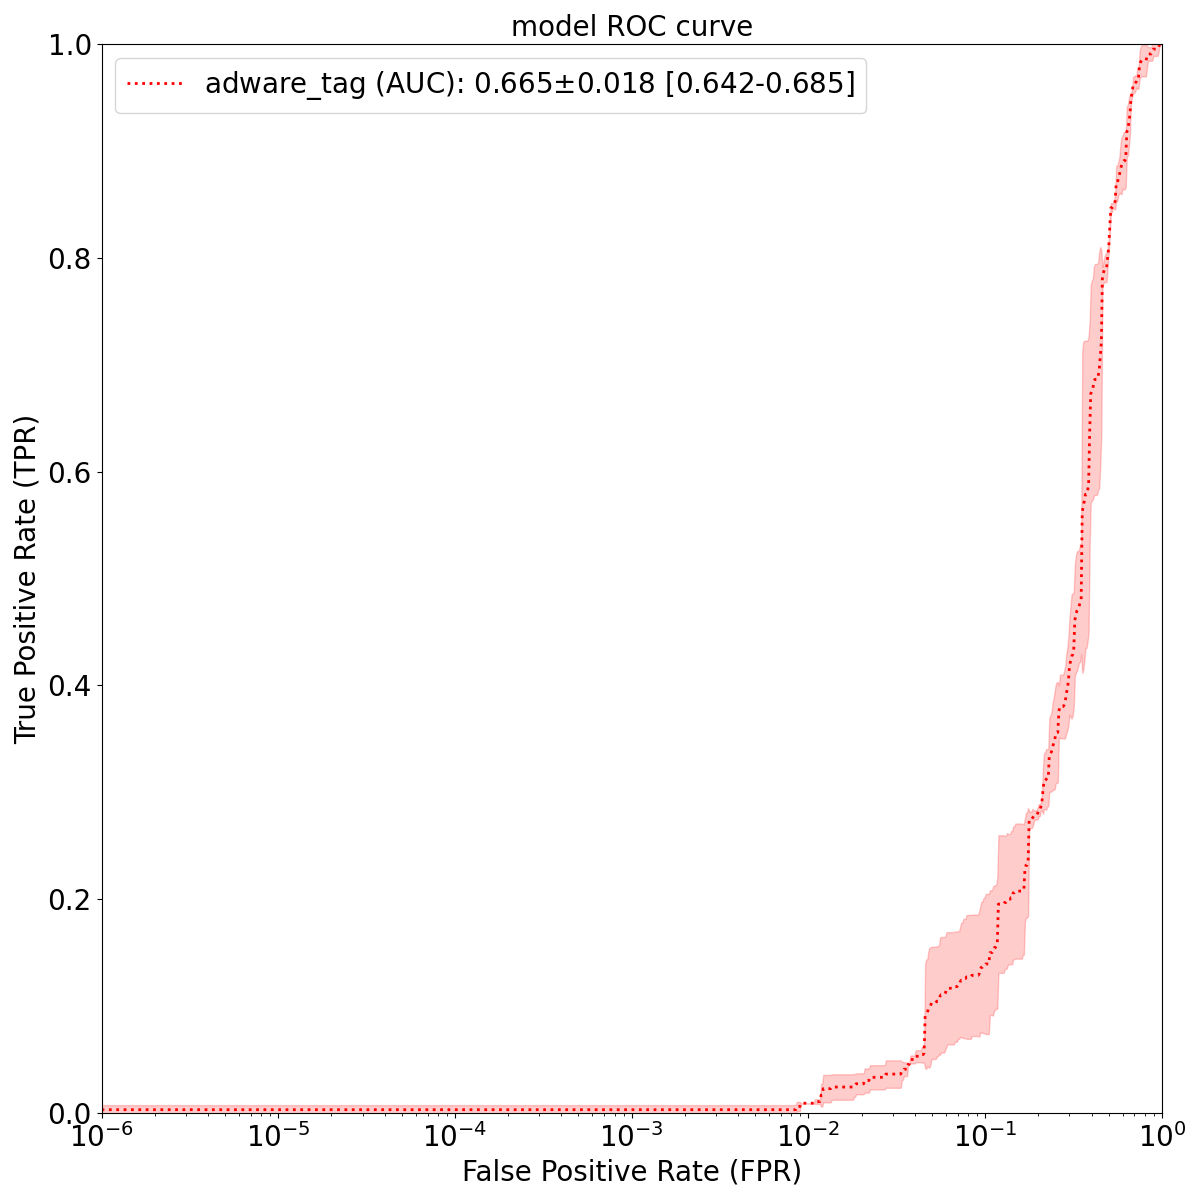
\includegraphics[width=0.6\textwidth]{./results/adware_tag_roc_aloha.png}
        \vspace*{-0.2cm}
        \caption{ROC curve and AUC statistics of \textBF{ALOHA} model for the \textbf{Adware Tag}. The line represents the \textit{mean} TPR at a given FPR, while the shaded region represents the \textit{standard deviation}. Statistics were computed over \textBF{3} training runs, each with random parameter initialization.}
        \label{fig:adwareTagRocAloha}
    \end{figure}
}

\newcommand{\adwareTagRocJointEmbedding}{
    \begin{figure}[H]
        \vspace*{-0.5cm}
        \centering
        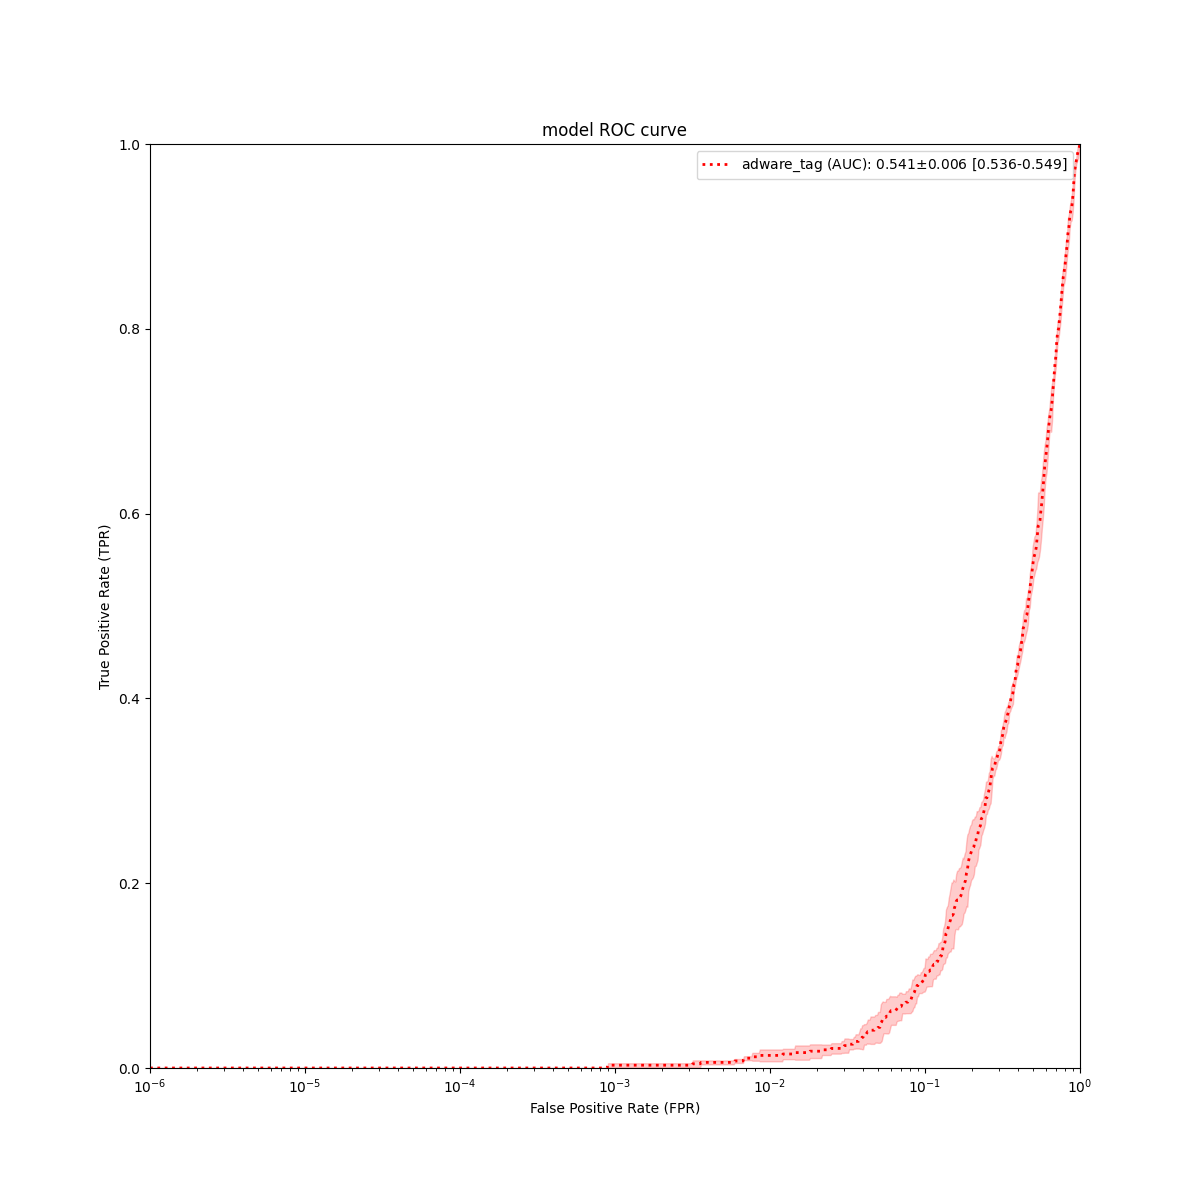
\includegraphics[width=0.6\textwidth]{./results/adware_tag_roc_jointEmbedding.png}
        \vspace*{-0.2cm}
        \caption{ROC curve and AUC statistics of \textBF{Joint Embedding} model for the \textbf{Adware Tag}. The line represents the \textit{mean} TPR at a given FPR, while the shaded region represents the \textit{standard deviation}. Statistics were computed over \textBF{3} training runs, each with random parameter initialization.}
        \label{fig:adwareTagRocJointEmbedding}
    \end{figure}
}

\newcommand{\adwareTagRocProposedMethod}{
    \begin{figure}[H]
        \vspace*{-0.5cm}
        \centering
        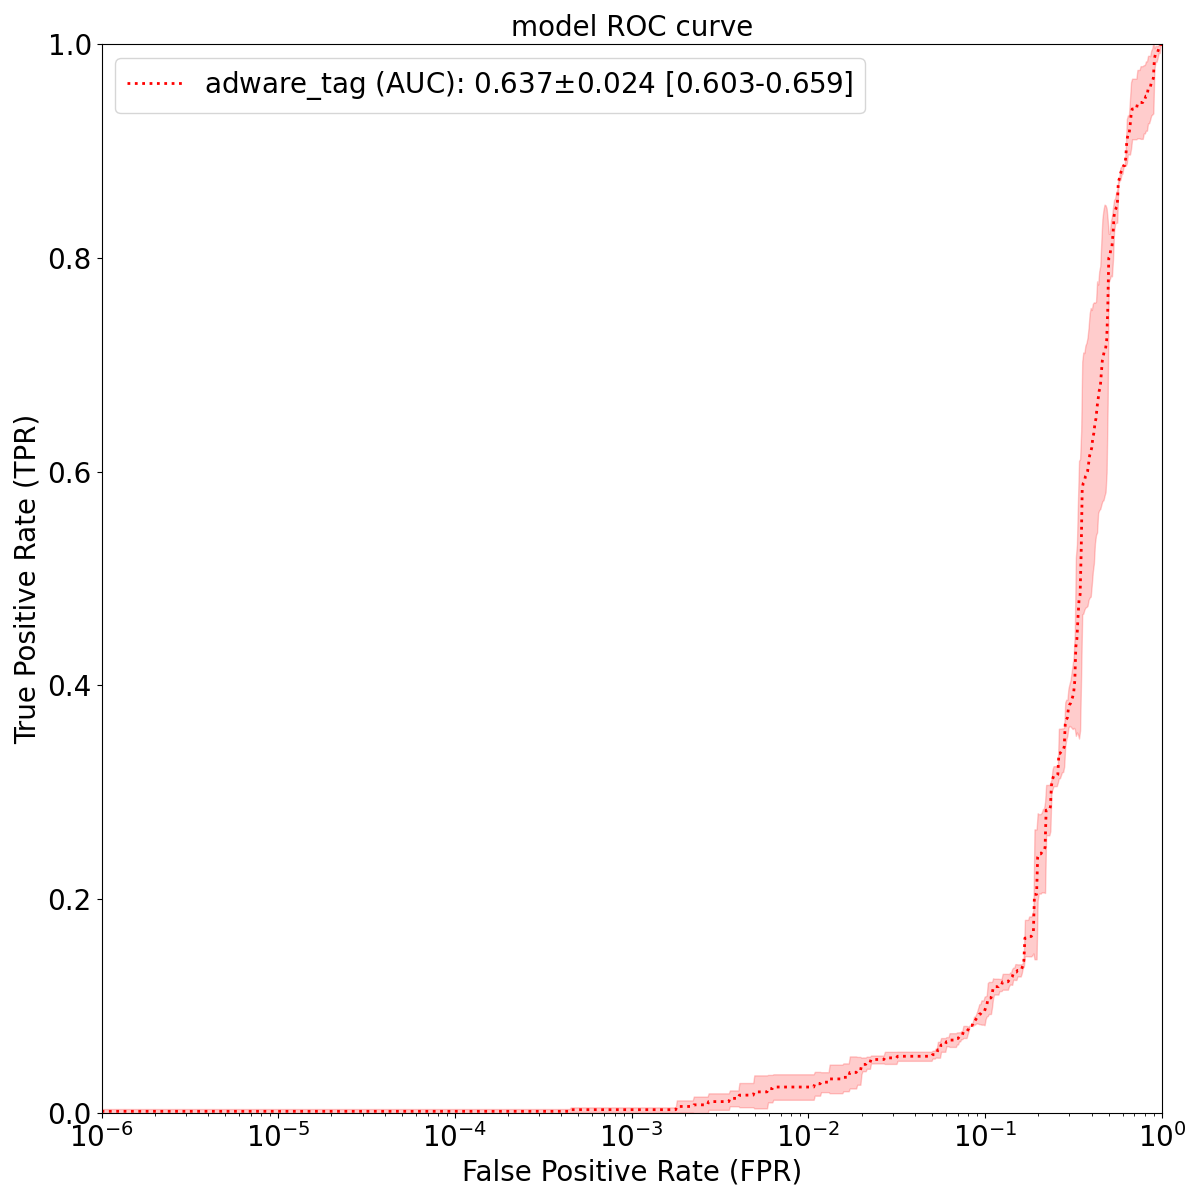
\includegraphics[width=0.6\textwidth]{./results/adware_tag_roc_proposedModel.png}
        \vspace*{-0.2cm}
        \caption{ROC curve and AUC statistics of \textBF{Proposed Model} for the \textbf{Adware Tag}. The line represents the \textit{mean} TPR at a given FPR, while the shaded region represents the \textit{standard deviation}. Statistics were computed over \textBF{3} training runs, each with random parameter initialization.}
        \label{fig:adwareTagRocProposedModel}
    \end{figure}
}
